\documentclass[12pt]{jsarticle}
\usepackage[top=30truemm,bottom=30truemm,left=25truemm,right=25truemm]{geometry}
\usepackage[dvipdfmx]{graphicx,color}
\usepackage{amsmath}
\usepackage{makeidx}
\usepackage{here}
\usepackage{nccmath}
\usepackage{url}
\usepackage{caption}
\usepackage{listings,jvlisting}
\usepackage{setspace}

\usepackage[skip=0cm,list=true,labelfont=it]{subcaption}
\linespread{1.12}
\graphicspath{{./images/}}

\AtBeginDocument{
  \abovedisplayskip     =1.8\abovedisplayskip
  \abovedisplayshortskip=1.8\abovedisplayshortskip
  \belowdisplayskip     =1.8\belowdisplayskip
  \belowdisplayshortskip=1.8\belowdisplayshortskip
}

\lstset{
  basicstyle={\ttfamily},
  identifierstyle={\small},
  commentstyle={\smallitshape},
  keywordstyle={\small\bfseries},
  ndkeywordstyle={\small},
  stringstyle={\small\ttfamily},
  frame={tb},
  breaklines=true,
  columns=[l]{fullflexible},
  numbers=left,
  xrightmargin=0zw,
  xleftmargin=3zw,
  numberstyle={\scriptsize},
  stepnumber=1,
  numbersep=1zw,
  lineskip=-0.5ex
}

\begin{document}

\begin{titlepage}
  \begin{center}
  \vspace*{70truept}

  {\huge 卒業論文}
  
  \vspace{30truept}
  
  \begin{spacing}{1.2}
    \huge タイトル
  \end{spacing}
  
  \vspace{150truept}

  {\LARGE 令和4年2月4日}

  \vspace{20truept}

  {\huge 神戸大学 工学部 市民工学科}

  \vspace{20truept}
  
  {\LARGE 学籍番号 1111111T}

  \vspace{20truept}

  {\huge 〇〇 〇〇}

  \vspace{50truept}

  {\LARGE 主査:〇〇 〇〇 准教授}

  \vspace{20truept}

  {\LARGE 副査:〇〇 〇〇 教授}
  
  \end{center}
  \end{titlepage}

  \clearpage

  \begin{center}
  \vspace*{50truept}
  
  \begin{spacing}{1.2}
    \LARGE English Title
  \end{spacing}
  
  \vspace{20truept}

  {\large 〇〇 〇〇}

  \vspace{10truept}

  {\large 1714214T}

  \vspace{10truept}
  
  {\large Department of Civil Engineering}

  \vspace{10truept}

  {\large Faculty of Engineering}

  \vspace{10truept}

  {\large Kobe University}

  \vspace{20truept}

  {\large February 4, 2022}

  \vspace{20truept}

  {\large ABSTRACT}
  
  \end{center}

  In this study, we ...

  \clearpage
  \tableofcontents
  \clearpage

  \section{序論}

  \subsection{研究背景と目的}

  近年では、

  \subsection{既往の研究}

  \subsubsection{既往研究a}

  既往研究aでは、...

  \paragraph{〇〇}

  \begin{figure}[H]
    \begin{center}
      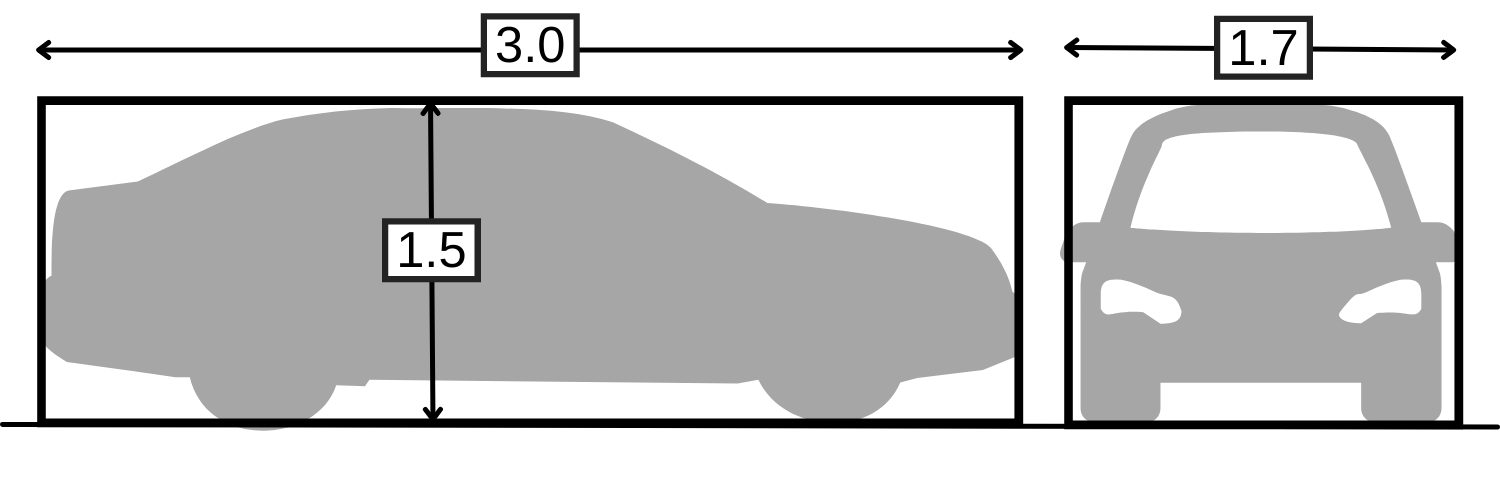
\includegraphics[width=10cm]{images/car_design.png}
    \end{center}
    \caption{
      車の寸法(m)
    }
    \label{fig:previous1_site_map}
  \end{figure}

  \paragraph{パラグラフ1}

  パラグラフ1では、...

  \paragraph{パラグラフ2}

  パラグラフ2では、...\\

  \subparagraph{サブパラグラフ1}

  サブパラグラフ1では、...

  \subparagraph{サブパラグラフ2}

  サブパラグラフ2では、...

  \paragraph{パラグラフ3}

  パラグラフ3では、...

  \section{実験方法}

  \subsection{サブセクション1}

  \begin{figure}[H]
    \begin{center}
      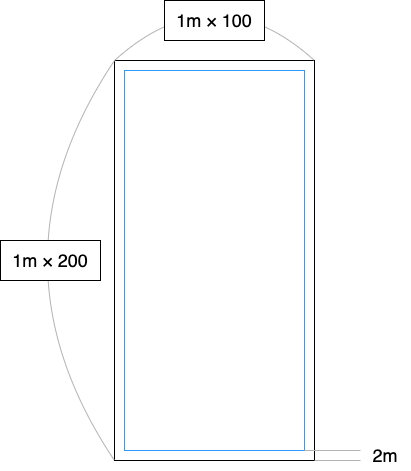
\includegraphics[width=7cm]{images/site_map.png}
    \end{center}
    \caption{研究対象サイト}
    \label{fig:site_map}
  \end{figure}

  \begin{figure}[H]
    \begin{center}
      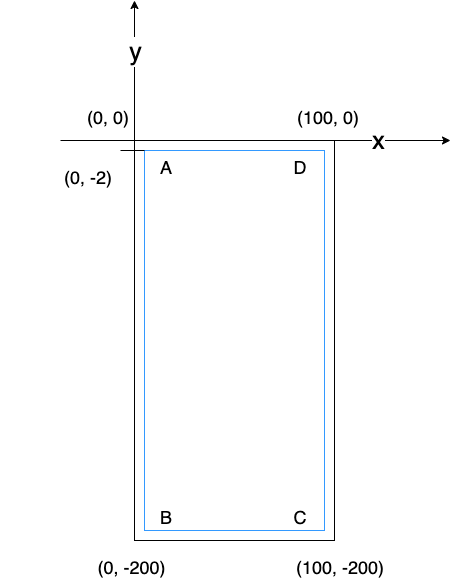
\includegraphics[width=6cm]{images/site_map_x_y.png}
    \end{center}
    \caption{xy軸に置いた研究対象サイト}
    \label{fig:site_map_x_y}
  \end{figure}

  サブセクション1では、...
  
  \subsection{サブセクション2}

  サブセクション1では、...

  \subsubsection{車両モデル}

  \begin{figure}[H]
    \begin{center}
      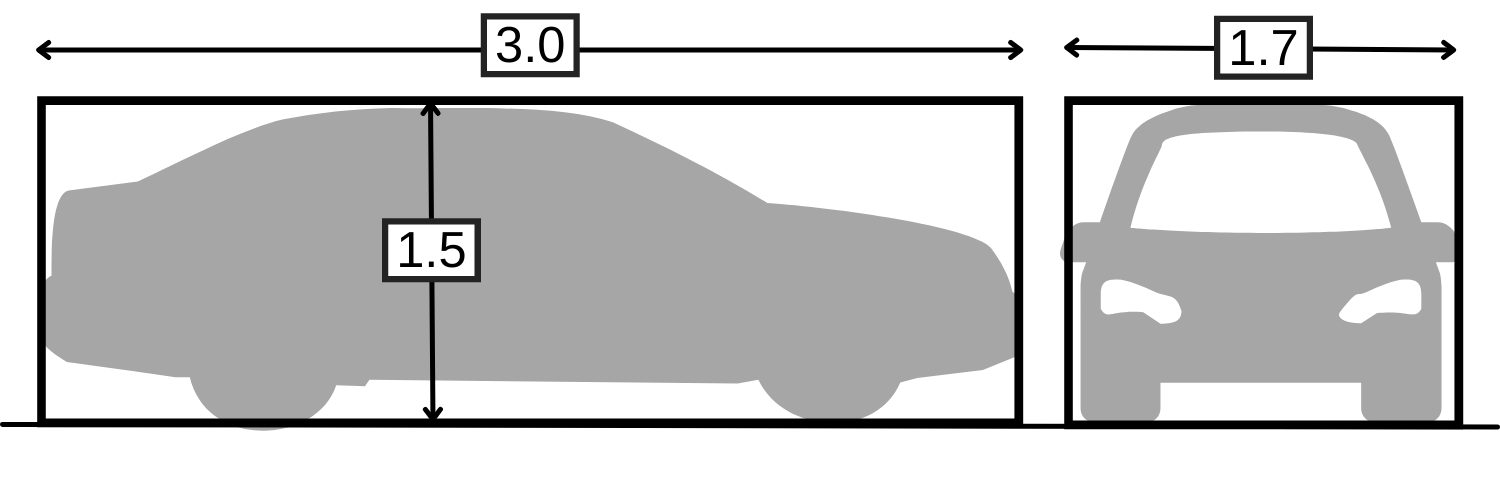
\includegraphics[width=10cm]{images/car_design.png}
    \end{center}
    \caption{車両の寸法(単位: m)}
    \label{fig:car_design}
  \end{figure}

  車両モデルの寸法は、

  \subsection{数値シミュレーション概要}

  数値シミュレーションでは、

  \subsubsection{氾濫解析}
  
  氾濫解析の際には、

  \paragraph{2次元堤内地計算}

  数式は以下のように記述します。

  \begin{align}
    &\frac{\partial h}{\partial t}
    +\frac{\partial M}{\partial x}
    +\frac{\partial N}{\partial y}
    =\frac{qDx_{dike}}{A_{cell}+r}\\
    &\frac{\partial M}{\partial t}
    +\frac{\partial uM}{\partial x}
    +\frac{\partial vM}{\partial y}
    =-gh\frac{\partial H}{\partial x}
    -gn^2u\frac{\sqrt{u^2+v^2}}{h^{\frac{1}{3}}}\\
    &\frac{\partial N}{\partial t}
    +\frac{\partial uN}{\partial x}
    +\frac{\partial vN}{\partial y}
    =-gh\frac{\partial H}{\partial y}
    -gn^2v\frac{\sqrt{u^2+v^2}}{h^{\frac{1}{3}}}
  \end{align}

  \noindent
  ここに、\(h\)は水深、
  \(n\)はマニング粗度係数、
  \(M=uh\)、
  \(N=vh\)であり、
  \(M\)、\(N\)は流量フラックス、
  \(u\)、\(v\)はそれぞれ\(x\)方向、
  \(y\)方向の流速、
  \(H\)は水位、
  \(r\)は降雨強度である。
  また、\(Dx_{dike}\)は1次元河道計算の節点間距離で
  \(A_{cell}\)は2次元堤内地計算のセル面積である。

  \subsubsection{車両または人型モデル流失計算}

  車体もしくは人体(以下漂流物とする)側方への抗力を\(D\)、抵抗力(漂流物と路面間の摩擦力)を\(F\)とする。
  ここで、流体力\(D\)と摩擦力\(F\)は次式で表される。

  \begin{align}
    &D=\rho AC_D\frac{v^2}{2}\\
    &F=\mu(W-B)
  \end{align}

  \noindent
  ここで、\(ρ\):密度、
  \(A\):投影面積、
  \(v\):流速、
  \(μ\):車両の静止摩擦係数、
  \(W\):漂流物の重力、
  \(B\):漂流物の浮力を表す。

  \begin{align}
    C_D=2.66-3.33\cdot\frac{h}{k}
  \end{align}

  \paragraph{条件に応じた流失計算}

  \noindent
  プログラムは以下のように記述します。

  \begin{lstlisting}[caption=流失計算のサンプルプログラム,label=losing_sample_program]
  for (jj = foo + 1; jj >= 2; jj--)
  {
      for (ii = 2; ii <= bar + 1; ii++)
      {
          // コメント
      }
  }
  \end{lstlisting}

  \noindent
  プログラム\ref{losing_sample_program}では、

  \subsection{実験ケース}

  \begin{figure}[H]
    \begin{center}
    \begin{minipage}[b]{0.45\linewidth}
      \centering
      
\includegraphics[width=5.5cm]{images/car_init.png}
      \subcaption{y軸と並行で正方向の流れ}
    \end{minipage}
    \begin{minipage}[b]{0.45\linewidth}
      \centering
      
\includegraphics[width=5.5cm]{images/diag_car_init.png}
      \subcaption{斜め流れ}
    \end{minipage}
    \end{center}
    \caption{各ケースの初期水深分布と漂流物の初期位置}
    \label{fig:car_init}
  \end{figure}

  実験ケースとしては以下のように2種類を用意した。

  \begin{enumerate}
    \item \textbf{ケース1}
    \item \textbf{ケース2}
  \end{enumerate}

  \noindent
  この際、

  \section{実験結果と考察}

  まず、ケース1のシミュレーション結果を図\ref{fig:car_case1_3m}に示す。

  \subsection{サブセクション1}

  \paragraph{ケース1}

  ケース1における氾濫状況の推移を把握するために、

  \begin{figure}[H]
    \begin{center}
    \begin{minipage}[b]{0.45\linewidth}
      \centering
      
\includegraphics[width=4.5cm]{images/diag_car_init.png}
      \subcaption{t=10s}
    \end{minipage}
    \begin{minipage}[b]{0.45\linewidth}
      \centering
      
\includegraphics[width=4.5cm]{images/diag_car_init.png}
      \subcaption{t=38s}
    \end{minipage}

    \begin{minipage}[b]{0.45\linewidth}
      \centering
      
\includegraphics[width=4.5cm]{images/diag_car_init.png}
      \subcaption{t=39s}
    \end{minipage}
    \begin{minipage}[b]{0.45\linewidth}
      \centering
      
\includegraphics[width=4.5cm]{images/diag_car_init.png}
      \subcaption{t=60s}
    \end{minipage}
    \end{center}
    \caption{初期水深3mの車両モデルケース1浸水シミュレーション結果}
    \label{fig:car_case1_3m}
  \end{figure}

  \begin{figure}[H]
    \begin{center}
      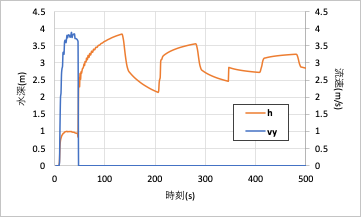
\includegraphics[width=8cm]{images/vy_h.png}
      \subcaption{水深-時刻と流速-時刻の関係}
      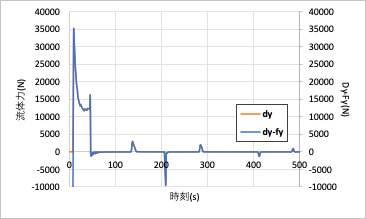
\includegraphics[width=8cm]{images/dy_dy_fy.png}
      \subcaption{流体力-時刻と\(D-F\)-時刻の関係}
    \end{center}
    \caption{初期水深3mの水深・
    流速(上)と車両への作用力(流体力\(D\)と\(D-F\)) (下)の時間変化}
    \label{fig:car_case1_3m_force}
  \end{figure}

  \noindent
  また、..である。

  \paragraph{ケース2}

  ケース2の計算結果を図\ref{fig:car_case3_2m}に示す。

  \subsection{サブセクション2}

  以下では、

  \paragraph{ケース1}

  \section{まとめ}

  本研究では、

  \addcontentsline{toc}{section}{\bibname}
  \begin{thebibliography}{99}
  \bibitem{a} 引用元a \url{https://github.com/TaKO8Ki}
  \bibitem{foo} 卒論太郎, 卒論太郎 引用元foo \url{https://github.com/TaKO8Ki}
  \bibitem{bar} 卒論太郎, 卒論太郎, 引用元bar
  \end{thebibliography}

  \clearpage

  背表紙
  
  令和3年度卒業論文 1111111T 〇〇〇〇
\end{document}
